\section{Illustration}
\subsection{Offline AIVC}
\label{sec:illust}
To illustrate the \aivcalg ~algorithm we use the example presented in Chapter \ref{ch:ivc} with $P = ({\small \texttt{on\_p}})$ .
%As inspired by the MARCO algorithm in \cite{marco2016fast}, we visualize $\mathcal{P}(\mathcal{A})$ as a lattice in a Hasse diagram (Figure~\ref{fig:lattice1}) to demonstrate the progress of the algorithm. As you can see, each level of the lattice contains sets with the same size linked to sets that are their immediate
%supersets (upper level regions) and subsets (lower level regions). Note that the power set is viewed as a Boolean formula, so each member in the lattice shows
% variable with $true$.
For better description, we view $T$ as an ordered set of its top-level conjuncts; i.e. $T = \{$ {\small \texttt{a1\_below, a2\_below, a1\_above, a2\_above, below, above\_hyst, doi\_on, d1, d2}} $\}$.
The algorithm starts with creating activation literals for each $T_i \in T$. Let the ordered set of Boolean variables $\{ a_1, \ldots , a_9 \}$ be the corresponding literals to the elements of $T$ (e.g. $\actlit ({ \small \texttt{a1\_below}}) = a_1$ and $\actlit ({\small \texttt{d2}}) = a_9$). Then, line 3 initializes $map$ with $\top$.

In the first iteration of the \texttt{while} loop, since $map$ is
empty, it is satisfiable, and a model for it can be any subset of
literals. So obviously, the first maximal model of $map$ contains all
the literals, which means, in line~\ref{alg:aivc:assignm}, $M = \{a_1,
\ldots, a_9\}$, and in line~\ref{alg:aivc:assigns}, $S = T$. Since $S$
is adequate for $P$, the \getivc ~module is called in
line~\ref{alg:aivc:getivc}. Suppose the returned \mivc\ by this function
is $S' = \{ { \small \texttt{a1\_below},~\texttt{below},
  ~\texttt{doi\_on}}\}$; this set is added to $A$ in
line~\ref{alg:aivc:addset}, and thus it comes to adding a new clause
to $map$ (line~\ref{alg:aivc:aadd}), which makes $map = (\neg a_1 \vee
\neg a_5 \vee \neg a_7)$. As discussed, this constraint
marks all the supersets of $S'$ as blocked and prunes them off the
search space.

%For the second iteration, $map$ is still satisfiable,
%so the algorithm gets to find a maximal model of it in line~\ref{alg:aivc:maxsat}. Suppose this time, the maximal model makes $M = \{a_1, \ldots, a_7\}$,
%which leads to $S = T \setminus \{ {\small \texttt{on\_p}}\} $ in line~\ref{alg:aivc:assigns}.
%Since $S$ is inadequate for $P$,
%the algorithm jumps to line 12 updating
%$map$ as $map \leftarrow map \wedge a_8$.
%Adding this new clause removes all the subsets of
%$T \setminus \{{\small \texttt{on\_p}}\}$
%from the search space. Similarly, in the third iteration,
%if the maximal model of $map$
For the second iteration, $map$ is still satisfiable,
so the algorithm gets to find a maximal model of it in line~\ref{alg:aivc:maxsat}. Suppose this time, the maximal model makes $M = \{a_1, \ldots, a_4, a_6, \ldots, a_9\}$, then $S = T \setminus \{ {\small \texttt{below}}\} $ will be another inadequate set that makes $map$ become
$map \leftarrow map \wedge a_5$
in line~\ref{alg:aivc:iadd}.

Suppose, in the third iteration, the maximal model leads to $M = \{a_2, \ldots, a_9\}$ and
$S = T \setminus \{ {\small \texttt{a1\_below}}\} $ in lines~\ref{alg:aivc:assignm} and~\ref{alg:aivc:assigns}.
Since this $S$ is adequate for $P$, \getivc ~computes a new \mivc\ in line~\ref{alg:aivc:getivc}.
Let the new \mivc\ be $S' = \{ {\small \texttt{a2\_below},~\texttt{below}, ~\texttt{doi\_on}}\}$; after adding this set to $A$,
it is time to constrain $map$ by a new clause in line~\ref{alg:aivc:addset},
which results in $map \leftarrow map \wedge (\neg a_2 \vee \neg a_5 \vee \neg a_7)$.

After these iterations, $map$ is still satisfiable, and the maximal model is
 $S = T \setminus \{ { \small \texttt{a1\_below}}, { \small \texttt{a2\_below}}\}$ in line~\ref{alg:aivc:assigns}.
In this case, $S$ is inadequate, so we update $map$ as
$map \leftarrow map \wedge (a_1 \vee a_2)$ (line~\ref{alg:aivc:iadd}). After adding this new clause to $map$,
all the subsets of $T \setminus \{ { \small \texttt{a1\_below}}, {\small \texttt{a2\_below}}\}$
will be blocked. The algorithm continues similar to the fourth iteration leading to $S$ (in line~\ref{alg:aivc:assigns}) and $map$ (in line~\ref{alg:aivc:iadd}) to be as
 $S = T \setminus \{ {\small  \texttt{doi\_on}}\}$ and $map \leftarrow map \wedge a_7$.

Finally, after the fifth iteration, $map$ becomes \unsat and the algorithm terminates.
Note that $MIS$es and $IVC$s may be discovered in different orders from what explained here. The order by which sets are explored is
quite dependent on the maximal model returned in line~\ref{alg:aivc:maxsat} as well as the \mivc returned in line~\ref{alg:aivc:getivc} because there could be several distinct maximal models (\mis es) and \mivc s. For this example with a $|T| = 9$ and $|\mathcal{P}(T)| = 2^9$, a brute force approach of power set exploration needs to look into 512  cases. However, the \aivcalg ~algorithm only explored 5 cases to cover the entire power set. %Depending on the order by which \mivc s and \mis es are discovered, the total cases to explore by the algorithm may change.
% All in all, it is fair to say the \aivcalg ~algorithm is  linear in the size of $T$.
%This issue could affect the performance of the algorithm as well.


\subsection{Online AIVC}
\begin{figure}[t]
\centering
  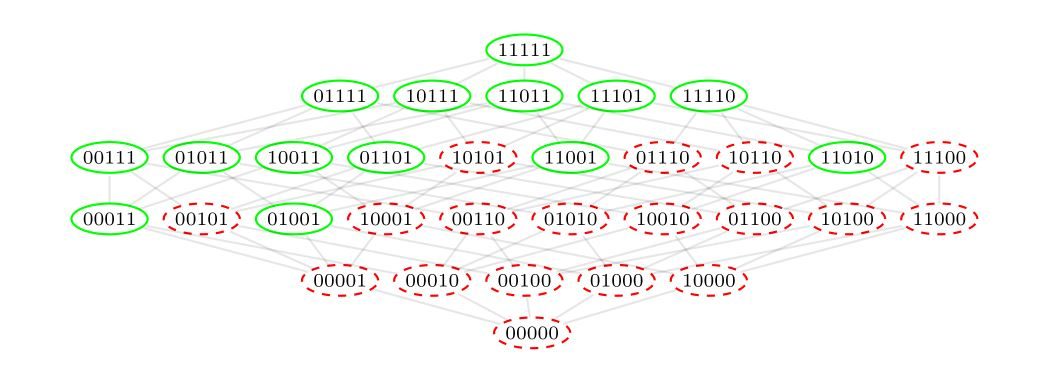
\includegraphics[width=\columnwidth]{figs/growshrink.jpg}
  \vspace{-0.1in}
\caption{The power set from the example execution of our algorithm.}
\label{fig:running_cube}
\end{figure}

The following example explains the execution of our algorithm on a simple instance where the transition step predicate $T$ is given as a conjunction of five sub-predicates $\{T_1, T_2, T_3, T_4, T_5\}$. We do not exactly state what are the predicates and what is the safety property of interest. Instead, Figure~\ref{fig:running_cube} illustrates the power set of $\{T_1, T_2, T_3, T_4, T_5\}$ together with an information about adequacy of individual subsets. The subsets with solid green border are the adequate subsets, and the subsets with dashed red border are the inadequate ones. To save space, we encode subsets as bitvectors, for example the subset $\{T_1, T_2, T_4\}$ is written as 11010. There~are~three~MIVCs~in~this example: 00011, 01001, and 11010.

We illustrate the first iteration of the main procedure \texttt{FindMIVCs} of our algorithm. Initially, all subsets are unexplored, i.e. $f_{\mathit{Unexplored}} = True$ and the queue $\mathit{shrinkingQueue}$ is empty. The procedure starts by finding a maximal unexplored subset and checking it for adequacy. In our case, $U_{\mathit{max}} = 11111$ is the only maximal unexplored subset and it is determined to be adequate. Thus, the algorithm \texttt{IVC\_UC} is used to compute an approximately minimal IVC $U_{\mathit{IVC}} = 01101$ which is then shrunk to a MIVC $01001$.

During the shrinking, sets $00101$, $01001$, and $01000$ are subsequently checked for adequacy and determined to be inadequate, adequate, and inadequate, respectively. The set $01001$ is the resultant MIVC, thus the formula $f_{\mathit{Unexplored}}$ is updated to $f_{\mathit{Unexplored}} = \mathit{True} \wedge (\neg x_2 \vee \neg x_5)$. The other two sets, $00101$ and $01000$, are enqueued to the $\mathit{growingQueue}$ and
grown at the end of the procedure.
%at the end of the procedure \texttt{Shrink}, they are grown.

We first grow the set $00101$. Initially, the procedure \texttt{Grow} picks $M = 10111$ as the maximal unexplored superset of $00101$, and checks it for adequacy. It is adequate and thus, an approximately minimal IVC $M_{\mathit{IVC}} = 00011$ is computed, enqueued to $\mathit{shrinkingQueue}$, and formula $f_{\mathit{Unexplored}}$ is updated to $f_{\mathit{Unexplored}} = \mathit{True} \wedge (\neg x_2 \vee \neg x_5) \wedge	(\neg x_4 \vee \neg x_5)$. Then, $M$ is (based on $M_{\mathit{IVC}}$) reduced to $M = 10101$ and checked for adequacy. It is found to be inadequate, thus formula $f_{\mathit{Unexplored}}$ is updated to $f_{\mathit{Unexplored}} = \mathit{True} \wedge (\neg x_2 \vee \neg x_5) \wedge	(\neg x_4 \vee \neg x_5) \wedge (x_2 \vee x_4)$, and the procedure terminates.

The growing of the set $01000$ results into an approximately maximal inadequate subset $01110$. Moreover, an approximately minimal IVC $11110$ is found during the growing and enqueued into $\mathit{shrinkingQueue}$. The formula $f_{\mathit{Unexplored}}$ is updated to $f_{\mathit{Unexplored}} = \mathit{True} \wedge (\neg x_2 \vee \neg x_5) \wedge	(\neg x_4 \vee \neg x_5) \wedge (x_2 \vee x_4) \wedge (\neg x_1 \vee \neg x_2 \vee \neg x_3 \vee \neg x_4) \wedge (x_1 \vee x_5)$.

After the second grow, the procedure \texttt{Shrink} terminates and the main procedure \texttt{FindMIVCs} continues. The queue $\mathit{shrinkingQueue}$ contains two sets: $00011$, $11110$, thus the procedure now shrinks them. During shrinking the set $00011$, the algorithm would attempt to check the sets $00001$ and $00010$ for adequacy, however since both these are already explored, the set $00011$ is identified to be a MIVC without performing any adequacy checks. The procedure \texttt{FindMIVCs} would now shrink also the set $11110$, thus empty the queue $\mathit{shrinkingQueue}$, and continue with a next iteration.
